\documentclass[a4paper,12pt]{article}
\usepackage{ucs}
\usepackage[utf8x]{inputenc}
\usepackage{amsfonts}
\usepackage[english,russian]{babel}
\usepackage[T1, T2A]{fontenc}
\frenchspacing
\usepackage{amsmath,amssymb,amsthm}
\usepackage[a4paper, margin=1in]{geometry}
\usepackage{fontspec}
\usepackage{noto}
\usepackage[table]{xcolor}
\usepackage{multirow}
\usepackage{diagbox}
\usepackage{graphicx}
\usepackage{listings}
\usepackage{minted}
\usepackage[obeyspaces]{xurl}
\usepackage{hyperref}
\usepackage{bm}
\usepackage{pdfpages}
\graphicspath{ {./img/} }
\renewcommand{\baselinestretch}{1.1}
\renewcommand{\arraystretch}{1.1}


\newtheorem{name}{Printed output}
\newtheorem{problem}{Задача}
\newenvironment{solution}{\renewcommand{\proofname}{\unskip\indent\nopunct}\begin{proof}}{\end{proof}}

\numberwithin{equation}{section}


\begin{document}

\sloppy




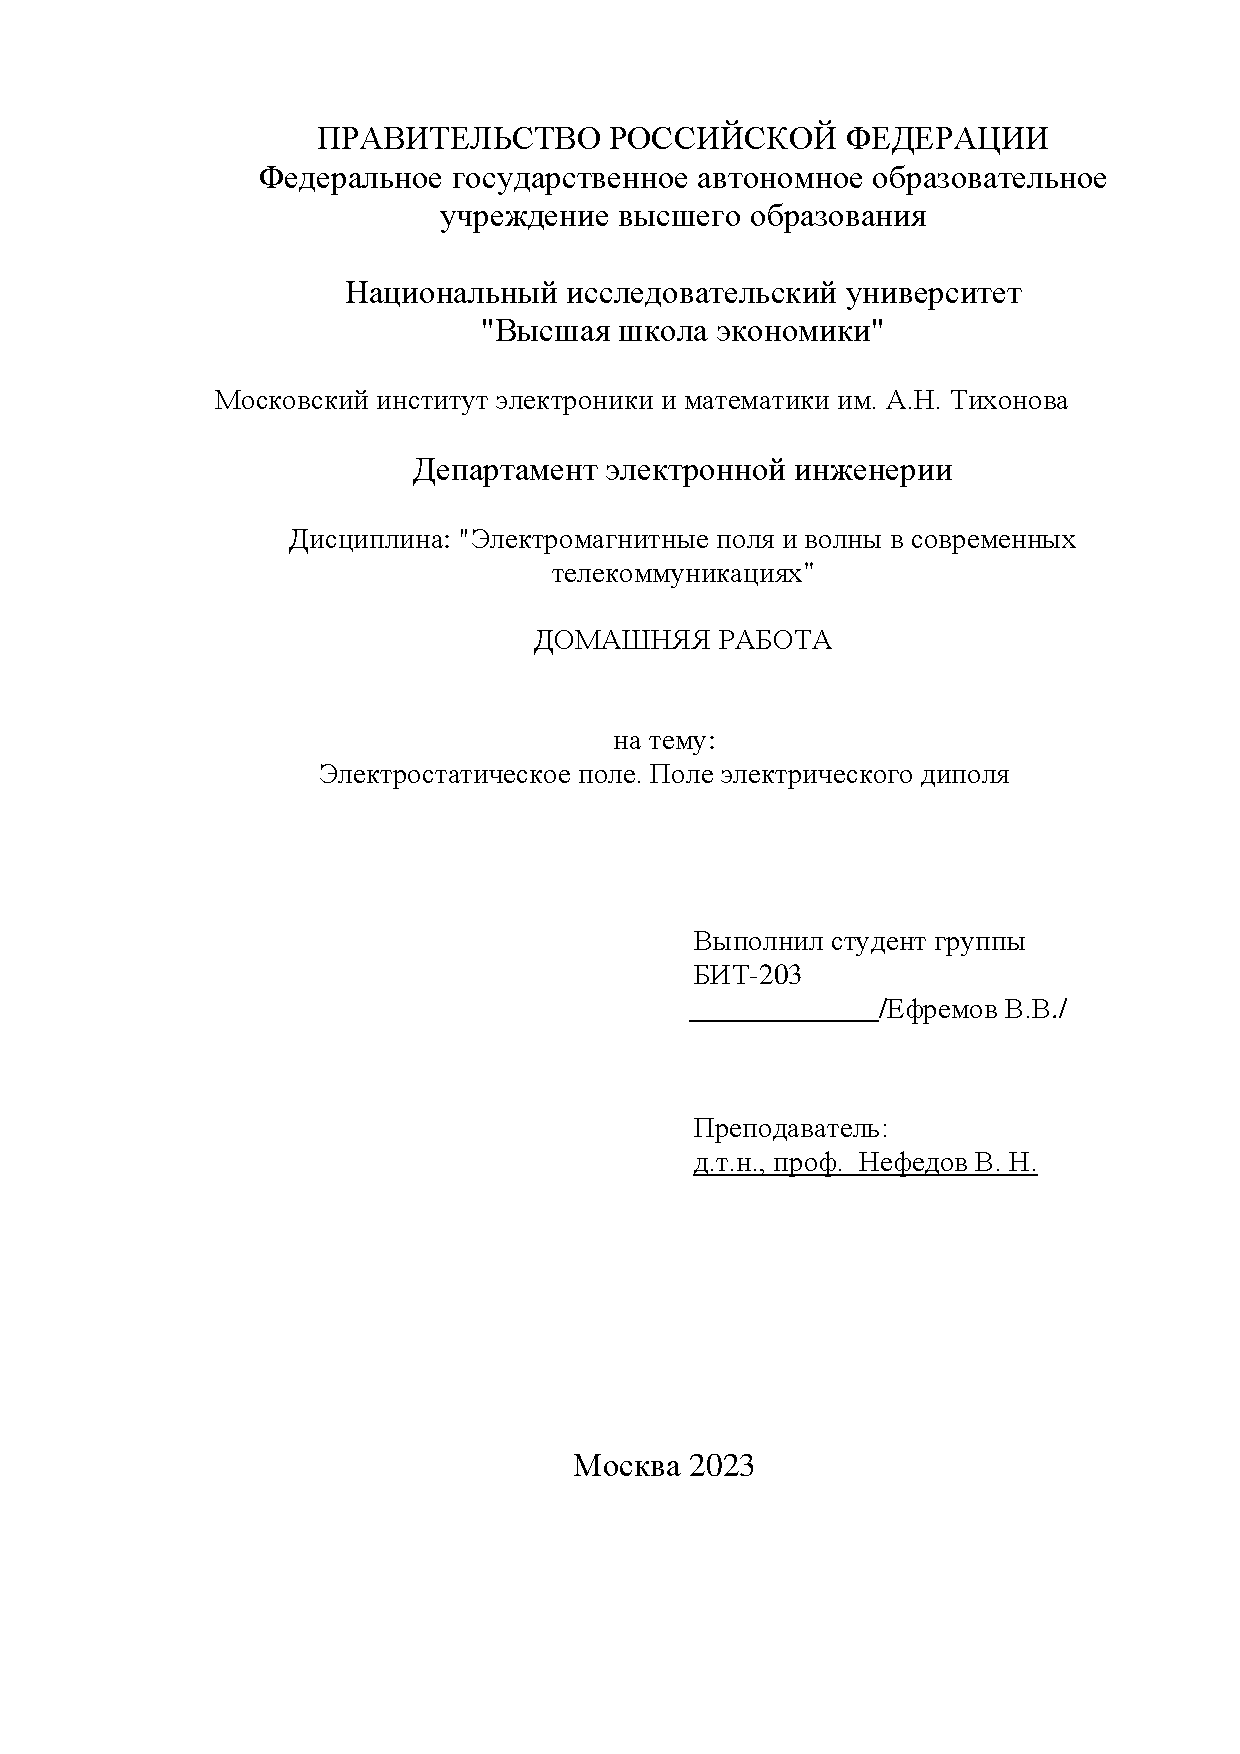
\includepdf[pages=-]{title.pdf}

\tableofcontents




\section{Введение}

Электромагнитное поле описывается уравнениями Максвелла.
Стоит отметить, что, во-первых, уравнения зависят от системы единиц измерения (в документе используется СИ, в СГС формулировки несколько отличаются).
Во-вторых, уравнения \ref{eq:mic} и \ref{eq:mac} эквивалентны.
Первый набор уравнений порой называют микроскопическими или уравнениями в вакууме, а второй - макроскопическими или уравнениями в среде.
Разница в том, что, в некотором смысле, второй набор уравнений зашивает свойства окружающей среды в поле.

\begin{subequations}
\label{eq:mic}
Уравнения Максвелла, в вакууме:
\begin{align}
        \nabla \cdot \bm{E} &= \frac{\rho}{\varepsilon_0} \label{eq:mica} \\
        \nabla \cdot \bm{B} &= 0 \label{eq:micb} \\
        \nabla \times \bm{E} &= -\frac{\partial{\bm{B}}}{\partial{t}} \label{eq:micc} \\
        \nabla \times \bm{B} &= \mu_0 \left(\bm{J} +\varepsilon_0 \frac{\partial{\bm{E}}}{\partial{t}}\right) \label{eq:micd}
\end{align}
\end{subequations}

\begin{subequations}
\label{eq:mac}
Уравнения Максвелла, в среде:
\begin{align}
        \nabla \cdot \bm{D} &= \rho \label{eq:maca} \\
        \nabla \cdot \bm{B} &= 0 \label{eq:macb} \\
        \nabla \times \bm{E} &= -\frac{\partial{\bm{B}}}{\partial{t}} \label{eq:macc} \\
        \nabla \times \bm{H} &= \bm{J} + \frac{\partial{\bm{D}}}{\partial{t}}\label{eq:macd}
\end{align}
\end{subequations}

Остановимся на обозначениях.
$\bm{E}$ - вектор напряженности электрического поля.
Показывает с какой силой поле будет действовать на пробный заряд.
Измеряется в В/м.

$\bm{D}$ - электрическая индукция, измеряется в $\text{Кл/м}^2$.
\begin{equation}
    \bm{D} = \varepsilon_0 \bm{E} + \bm{P}
\end{equation}
где $\bm{P}$ - вектор поляризации.
Зачастую можно считать, что вектор поляризации $\bm{P}$ пропорционален вектору напряженности электрического поля $\bm{E}$.
И тогда $\bm{D} = \varepsilon \bm{E}$.

$\bm{B}$ - вектор магнитной индукции.
Показывает с какой силой магнитное поле будет действовать на движущийся пробный заряд.
Единица измерения - тесла (Тл).

$\bm{H}$ - напряженность магнитного поля, измеряется в А/м.
\begin{equation}
    \bm{H} = \frac{1}{\mu_0} \bm{B} - \bm{M}
\end{equation}
где $\bm{M}$ - намагниченность.
В простейших случаях $\bm{M}$ пропорционален $\bm{B}$, откуда получается $\bm{B} = \mu_0 \mu \bm{H}$.

$\rho$ - плотность зарядов, измеряется в $\text{Кл/м}^3$.
$\bm{J}$ - плотность тока, измеряется в $\text{А/м}^2$.




\section{Электростатическое поле}

Электростатическое поле - поле неподвижных зарядов, или, если говорить точнее, случай когда плотность зарядов $\rho$ не меняется во времени.
Из-за стационарности во времени правые части всех уравнений кроме первого обнуляются.

Известно, что ротор градиента любой достаточно гладкой функции - нуль.
Поэтому можно написать $\bm{E} = \nabla \phi$.
Иногда такая запись оказывается полезной, т.к. сводит нахождение векторного поля $\bm{E}$ к поиску скалярного.

При такой замене уравнение \ref{eq:mica} превращается в
\begin{equation}
    \Delta \phi = \frac{\rho}{\varepsilon_0}
\end{equation}

Если взять уравнение \ref{eq:mica}, проинтегрировать по некоторому объему и применить теорему Стокса, то получится иногда полезное выражение
\begin{equation}
    \label{eq:gauss}
    \oint_{\partial V} \bm{E} \cdot d\bm{S} = \frac{1}{\varepsilon_0} \int_{V} \rho dV = \frac{Q}{\varepsilon_0}
\end{equation}
Т.е. интеграл по \textit{произвольной} замкнутой поверхности от напряженности электрического поля равен нормированной на $\varepsilon_0$ сумме зарядов внутри объема ограниченного поверхностью.




\section{Поле электрического диполя}

Рассмотрим действие электрического поля на атом.
Поле толкает положительно заряженную часть (ядро) в одну сторону и тянет отрицательно заряженную (облако электронов) в другую.
В результате атом как бы растягивается и поворачивается.
Этот эффект называется поляризацией, но давайте посмотрим на упрощенную модель - диполь.

(Физический) диполь - система из двух равных по величине и противоположных по знаку зарядов расположенных на малом расстоянии друг от дргуа.
Взаимодействие диполя с электрическим полем описывается дипольным моментом 
\begin{equation}
    \bm{p} = q \bm{d}
\end{equation}
Это вектор с направлением от отрицательного конца к положительному и длинной пропорциональной заряду.
Если вектора $\bm{E}$ и $\bm{p}$ не параллельны, то есть ненулевой момент силы, который заворачивает диполь.

Порой рассматривают идеальный диполь.
Он отличается от физического тем, что расстояние $d$ между зарядами устремлено к нулю, и, Соответственно, заряды устремлены к бесконечности чтобы сохранить конечный дипольный момент.

Если говорить о поле диполя, то его потенциал (в сферических координатах) имеет вид
\begin{equation}
    \phi_{dip} = \frac{p cos \theta}{4 \pi \varepsilon_0 r^2}
\end{equation}
А само поле
\begin{equation}\label{eq:3.3}
    \bm{E_{dip}} = \frac{p}{4 \pi \varepsilon_0 r^3} \left( 2 cos \theta \bm{r} + sin \theta \bm{\theta} \right)
\end{equation}

Стоит отметить, что потенциал диполя убывает как $r^{-2}$.
Для сравнения, потенциал точечного заряда убывает как $r^{-1}$.
Соответственно, напряженность поля диполя убывает как куб, а точечного заряда как квадрат.
Эта закономерность продолжается, если рассмотреть более сложные аналоги диполя - квадруполь (система из четырех зарядов в вершинах квадрата, потенциал убывает как $r^{-3}$), октополь (восемь зарядов расположенных в вершинах куба, потенциал убывает как $r^{-4}$).




\section{Примеры задач}

\begin{problem}
{\normalfont \cite[p.~76, Problem 2.12]{Griffiths:1492149}}
Найдите напряженность электрического поля внутри равномерно заряженного шара с плотностью заряда $\rho$.
\end{problem}
\begin{solution}
В этой задаче крайне полезна формула \ref{eq:gauss}.
Из-за сферической симметрии вектор напряженности $\bm{E}$ может зависеть только от расстояния до центра шара.
Возьмем в качестве области $V$ шар радиуса $r$.
Т.к. $E$ постоянна на границе шара, то интеграл по границе - это просто произведение $E$ на площадь границы.
\begin{equation}
    \oint_{\partial V} \bm{E} \cdot d\bm{S} = E(r) \cdot (4 \pi r^2) = \\
    \frac{1}{\varepsilon_0} \int_{V} \rho dV = \frac{4 \pi r^3 \rho}{3 \varepsilon_0}
\end{equation}
Откуда
\begin{equation}
    \bm{E}(\bm{r}) = \frac{\rho \bm{r}}{3 \varepsilon_0}
\end{equation}
\end{solution}


\begin{problem}
    {\normalfont \cite[p.~76, Problem 2.18]{Griffiths:1492149}}
    Два шара радиуса $R$ каждый равномерно заряжены с плотностями заряда $+\rho$ и $-\rho$ и расположены так, что частично пересекаются.
    Покажите что в области пересечения поле постоянно и найдите его значение.
\end{problem}
\begin{solution}
\begin{center}
    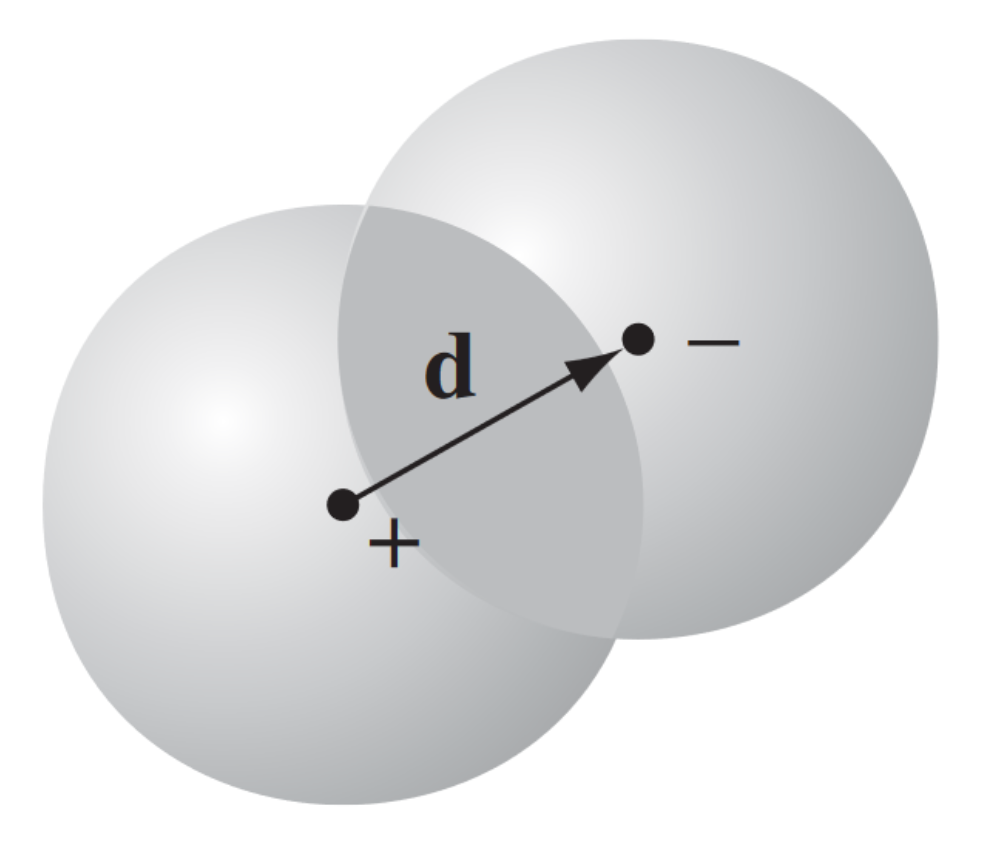
\includegraphics[width=5cm]{1.png}
\end{center}
Возьмем произвольную точку в пересечении и обозначим $\bm{r_+}$ и $\bm{r_-}$~- радиус-вектора до этой точки из центров шаров.
Поля создаваемые каждым из шаров известны из предыдущей задачи $\bm{E_+}(\bm{r_+}) = \frac{\rho \bm{r_+}}{3 \varepsilon_0}$, $\bm{E_-}(\bm{r_-}) = \frac{\rho \bm{r_-}}{3 \varepsilon_0}$.
И ответом будет их суперпозиция.
\begin{equation}
    \bm{E}(\bm{r}) = \frac{(\bm{r_+} - \bm{r_-}) \rho}{3 \varepsilon_0} = \frac{\rho \bm{d}}{3 \varepsilon_0}
\end{equation}
Где $\bm{d}$ - вектор от центра положительно заряженного шара до центра отрицательно заряженного.
\end{solution}


\begin{problem}
    {\normalfont \cite[p.~164, Problem 3.50(a)]{Griffiths:1492149}}
    Пусть распределение зарядов $\rho_1$ создает потенциал $\phi_1$, а заряды $\rho_2$ - $\phi_2$.
    Покажите что
\begin{equation}
    \int_{R^3} \rho_1 \phi_2 dV = \int_{R^3} \phi_1 \rho_2 dV
\end{equation}
\end{problem}
\begin{solution}
Докажем одно вспомогательное утверждение.
Пусть $f$ и $g$ - скалярные поля, тогда
\begin{equation}
    \nabla \cdot (f \nabla g) = \nabla f \cdot \nabla g + f \Delta g
\end{equation}
Действительно,
\begin{multline}
    \nabla \cdot (f \nabla g) = \nabla \cdot \left( f \sum_i \frac{\partial g}{\partial x_i} \bm{x_i} \right) =
    \sum_i \frac{\partial}{\partial x_i} \left( f \frac{\partial g}{\partial x_i} \right) = \\
    \sum_i \left( \frac{\partial f}{\partial x_i} \frac{\partial g}{\partial x_i} + f \frac{\partial^2 g}{\partial x_i^2} \right) =
    \nabla f \cdot \nabla g + f \Delta g
\end{multline}
Перейдем теперь к исходной задаче.
Рассмотрим следующий интеграл
\begin{multline}\label{eq:p3}
    \int \bm{E_1} \cdot \bm{E_2} dV = \int \nabla \phi_1 \cdot \nabla \phi_2 dV =
    \int \left( \nabla \cdot (\phi_1 \nabla \phi_2) - \phi_1 \Delta \phi_2 \right) dV = \\
    \int_{\partial V} \phi_1 \nabla \phi_2 dS - \int_V \phi_1 \Delta \phi_2 dV =
    - \int_V \phi_1 \frac{\rho_2}{\varepsilon_0} dV
\end{multline}
Здесь стоит пояснить почему интеграл по границе обращается в нуль.
Мы интегрируем по всему пространству, поэтому граница - это бесконечно удаленные точки.
Потенциал определяется с точностью до аддитивной константы и мы, для удобства, берем константу такой, чтобы на бесконечности потенциал обращался в нуль.

С другой стороны, все выкладки в \ref{eq:p3} симметричны относительно 1 и 2.
Поэтому, домножая на $-\varepsilon_0$, получаем
\begin{equation}
    \int_{R^3} \rho_1 \phi_2 dV = \int_{R^3} \phi_1 \rho_2 dV
\end{equation}
\end{solution}


\begin{problem}
    {\normalfont \cite[p.~166, Problem 3.56]{Griffiths:1492149}}
    Идеальный электрический диполь расположен в начале координат и направлен вверх (по оси $Oz$).
    Под действием поля диполя покоящийся точечный заряд расположенный на плоскости $xOy$ начинает двигаться.
    Покажите что он будет двигаться по полукруглой траектории подобно маятнику.
    \begin{center}
        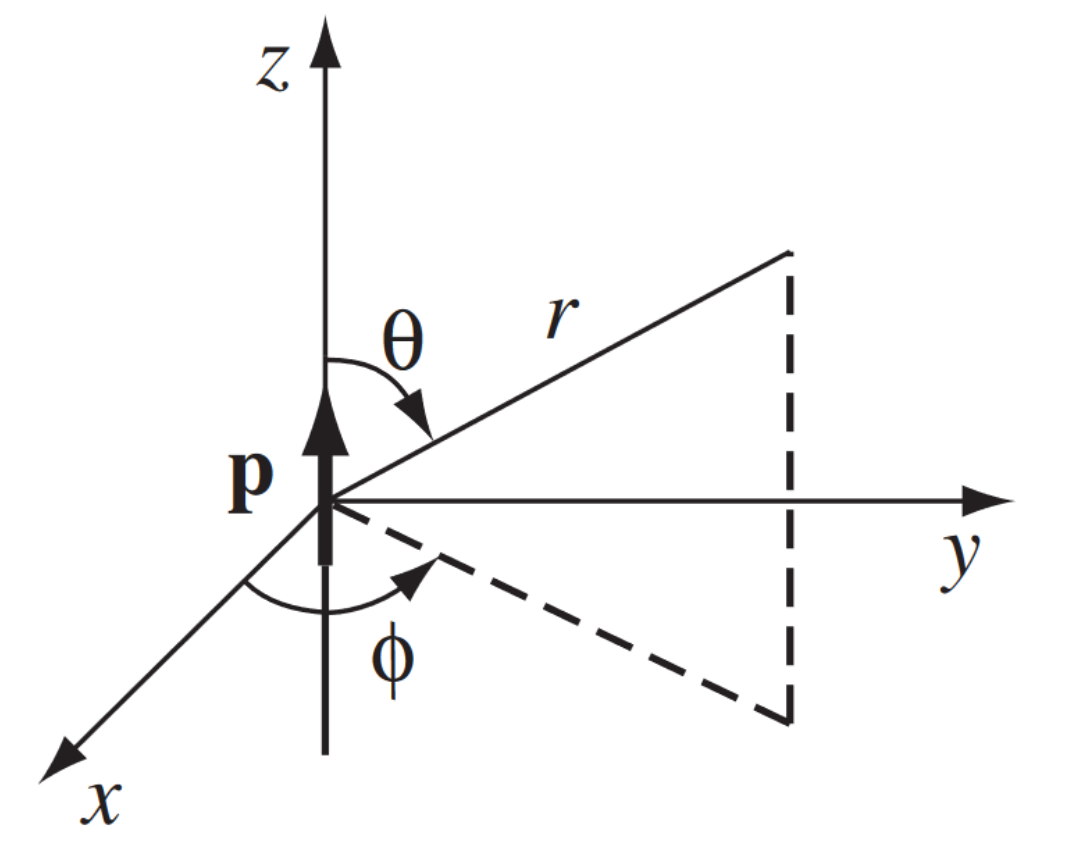
\includegraphics[width=5cm]{2.png}
    \end{center}
\end{problem}
\begin{solution}
Из \ref{eq:3.3} следует, что на заряд будет действовать сила
\begin{equation}\label{eq:4.9}
    \bm{F} = \frac{q p}{4 \pi \varepsilon_0 r^3} \left( 2 cos \theta \bm{r} + sin \theta \bm{\theta} \right)
\end{equation}

Рассмотрим математический маятник и покажем, что в нем, с точностью до константы, сила такая же.

\begin{center}
    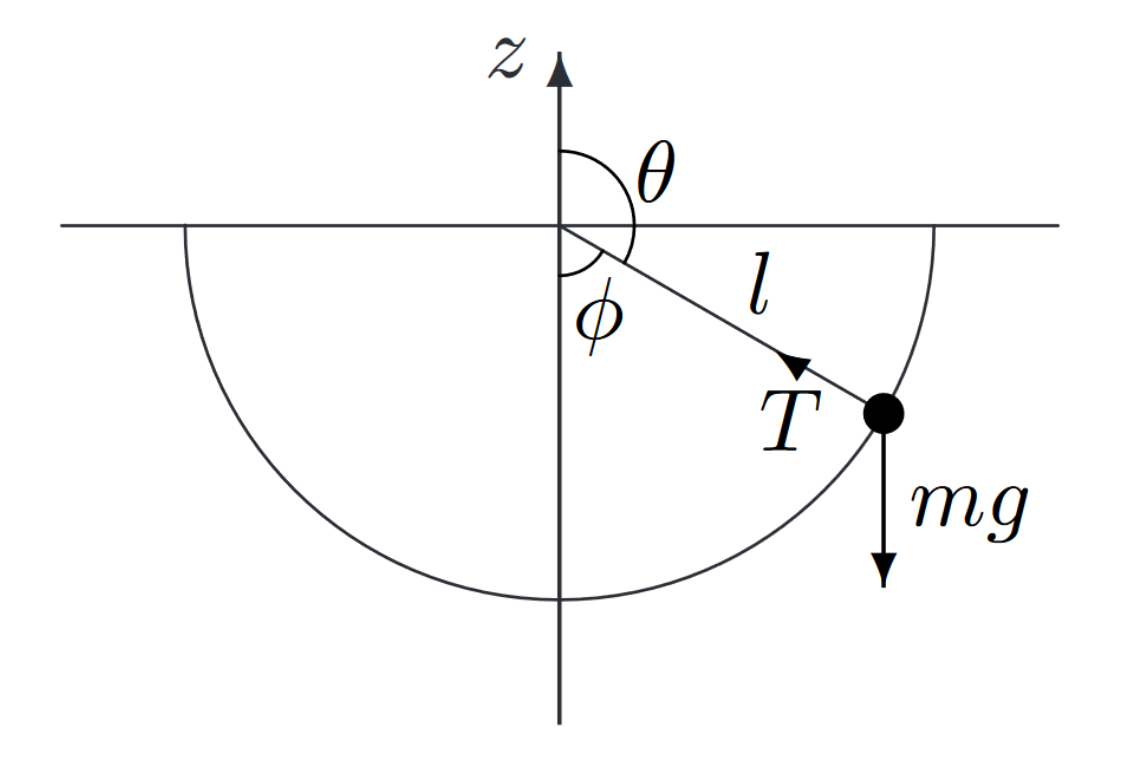
\includegraphics[width=8cm]{3.png}
\end{center}

Прежде всего, из закона сохранения энергии получается
\begin{equation}\label{eq:4.10}
    mgl cos \phi = \frac{mv^2}{2}
\end{equation}

Из второго закона Ньютона (в проекции на радиальную ось)
\begin{equation}\label{eq:4.11}
    m \frac{v^2}{l} = T - mg cos \phi
\end{equation}

Выражая $T$ из \ref{eq:4.11} и подставляя $v^2$ из \ref{eq:4.10}, получаем
\begin{equation}
    T = 3mg cos \phi = -3mg cos \theta
\end{equation}

На маятник действует всего две силы - тяжести и натяжения подвеса.
Суммарная сила действующая на маятник
\begin{equation}\label{eq:4.13}
    \bm{F} = -T \bm{r} - mg \bm{z} = 3mg cos \theta \bm{r} - mg \left( cos \theta \bm{r} - sin \theta \bm{\theta} \right) =
    mg (2 cos \theta \bm{r} + sin \theta \bm{\theta})
\end{equation}
Выражения \ref{eq:4.9} и \ref{eq:4.13} очень похожи, они отличаются только константой.
Первое описывает силу, которая действует на заряд в поле диполя, а второе - силу действующую на маятник.
Т.к. силы одинаковы, то и траектории будут одинаковы.
Поистине прелестный результат!
\end{solution}


\section{Литература}
\renewcommand\refname{\vskip -1cm}
\bibliographystyle{plain}
\bibliography{refs}




\end{document}
